\section{Procédés}

Voilà ci-dessous les nomenclatures ressources des différents produits.

	\begin{figure}[H]
\centering
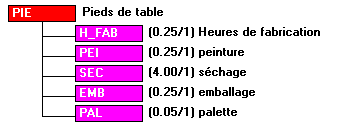
\includegraphics[scale=0.35]{./captures/pied.PNG}
\caption{Nomenclature du bloc}
	\end{figure}	
	
		\begin{figure}[H]
\centering
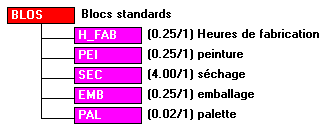
\includegraphics[scale=0.35]{./captures/standard.PNG}
\caption{Nomenclature du bloc}
	\end{figure}	
	
	
		\begin{figure}[H]
\centering
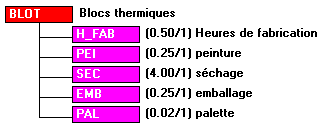
\includegraphics[scale=0.35]{./captures/thermique.PNG}
\caption{Nomenclature du bloc}
	\end{figure}	

Les blocs, tout comme les pieds, sont d'abord découpés sur une planche. Il sont ensuite travaillés sur la forme, avant d'être peints puis séchés. Ils sont finalement emballés et organisés sur des palettes pour la livraison aux entreprises.
